%!TEX root = ../report.tex

\chapter{Features of simulation instances}
\label{appendix:features}

The following sections provide the two set of simulation instance features used in the study.

\section{Dataset creation and experimental setup instance}
\label{section:feature_table_training}
The table \ref{table:simulationinstances_train} provides the features of the simulation instances used for training and experiments. This set of 16 instances are used to generate the dataset for training the cost and configuration response models. Each instance is optimized using SMAC for 100 iterations and results in  1600 (16 $\times$ 100) observations comprising the dataset. The experiments include the repeatability test of SMAC, the ability of SMAC to outperform the current default configurations and the behavior of SMAC for different iterations utilize the instances with the features provided in the table \ref{table:simulationinstances_train}. The table \ref{table:simulationinstances_train} is referred in the previous chapter \ref{chapter:experimentation_results}.

\section{Unseen simulation instances}
\label{section:feature_table_evaluation}

The features of the three simulation instances are provided in table \ref{table:simulationinstances_evaluation}. This feature set is used in section \ref{section:real_eval} to evaluate the predictions from the smart coupling tool.

\begin{landscape}
\begin{table}[]
\begin{tabular}{|l|l|l|l|l|l|l|l|}
\hline
\textbf{Instance}  &\multicolumn{1}{|p{2cm}|}{\centering \textbf{Simulation \\problem}}
 & \multicolumn{1}{|p{2cm}|}{\centering \textbf{Solid-Fluid\\density ratio}} 
& \multicolumn{1}{p{2cm}|}{\centering \textbf{Fluid –\\ density ($kg/m^3$)}}
& \multicolumn{1}{p{2cm}|}{\centering \textbf{\centering Solid –\\ elasticity (Pascal)}}
& \multicolumn{1}{p{2cm}|}{\centering \textbf{Poisson's ratio}}
& \multicolumn{1}{p{2cm}|}{\centering \textbf{Fluid – viscosity (Pascal second)}}
& \multicolumn{1}{p{2cm}|}{\centering \textbf{Time step (second)}} \\ \hline
1 &3D driven cavity & 2.50E+02 & 1.00E+00 & 2.50E+02 & 0.00E+00 & 1.00E-03 & 1.00E-01 \\ \hline
2 & 3D driven cavity & 1.00E+02 & 1.00E+00 & 2.50E+02 & 0.00E+00 & 1.00E-03 & 1.00E-01 \\ \hline
3 & 3D driven cavity & 1.00E+02 & 1.00E+00 & 1.00E+03 & 0.00E+00 & 1.00E-03 & 1.00E-01 \\ \hline
4 & 3D driven cavity & 1.00E+02 & 1.00E+00 & 1.00E+04 & 0.00E+00 & 1.00E-03 & 1.00E-01 \\ \hline
5 & 3D driven cavity & 1.00E+01 & 1.00E+01 & 2.50E+02 & 0.00E+00 & 2.00E-04 & 1.00E-01 \\ \hline
6 & 3D driven cavity & 1.00E+02 & 1.00E+01 & 1.00E+03 & 0.00E+00 & 1.00E-03 & 1.00E-02 \\ \hline
7 & 3D driven cavity & 2.50E+01 & 1.00E+01 & 2.50E+02 & 0.00E+00 & 1.00E-03 & 2.00E-02 \\ \hline
8 & 3D driven cavity & 1.00E+01 & 1.00E+01 & 1.00E+03 & 0.00E+00 & 1.00E-03 & 2.00E-02 \\ \hline
9 & 3D driven cavity & 1.00E+01 & 1.00E+01 & 1.00E+04 & 0.00E+00 & 1.00E-03 & 2.00E-02 \\ \hline
10 & 3D driven cavity & 1.00E+01 & 1.00E+00 & 1.00E+04 & 0.00E+00 & 1.00E-03 & 2.00E-02 \\ \hline
11 & 3D driven cavity & 1.00E+01 & 1.00E+01 & 1.00E+04 & 0.00E+00 & 1.00E-03 & 2.00E-01 \\ \hline
12 &3D driven cavity & 1.00E+01 & 1.00E+02 & 1.00E+04 & 0.00E+00 & 1.00E-03 & 5.00E-02 \\ \hline
13 & 3D driven cavity & 1.00E+01 & 1.00E+02 & 1.00E+05 & 0.00E+00 & 1.00E-03 & 1.00E-02 \\ \hline
14 & Elastic flap & 1.00E+03 & 1.00E+00 & 1.00E+08 & 4.90E-01 & 2.00E-05 & 1.00E-04 \\ \hline
15 & Elastic flap& 1.00E+01 & 1.00E+02 & 1.00E+06 & 4.90E-01 & 2.00E-05 & 1.00E-04 \\ \hline
16 & Elastic flap & 1.00E+02 & 1.00E+01 & 1.00E+04 & 4.90E-01 & 2.00E-05 & 1.00E-04 \\ \hline
\end{tabular}
\captionsetup{justification=justified}
\caption[Features of simulation instances used for training and experiments]{Features of 16 simulation instances used for dataset collection and experiments.}
\label{table:simulationinstances_train}
\end{table}
\end{landscape}

\begin{landscape}
\begin{table}[]
\begin{tabular}{|l|l|l|l|l|l|l|l|}
\hline
\multicolumn{1}{|p{2cm}|}{\centering \textbf{Evaluation\\instance}} &\multicolumn{1}{|p{1.8cm}|}{\centering \textbf{Simulation \\problem}}
 & \multicolumn{1}{|p{1.8cm}|}{\centering \textbf{Solid-Fluid\\density ratio}} 
& \multicolumn{1}{p{1.8cm}|}{\centering \textbf{Fluid –\\ density ($kg/m^3$)}}
& \multicolumn{1}{p{1.9cm}|}{\centering \textbf{\centering Solid –\\ elasticity (Pascal)}}
& \multicolumn{1}{p{1.9cm}|}{\centering \textbf{Poisson's ratio}}
& \multicolumn{1}{p{1.9cm}|}{\centering \textbf{Fluid – viscosity (Pascal second)}}
& \multicolumn{1}{p{1.9cm}|}{\centering \textbf{Time step (second)}}  \\ \hline
1 & 3D driven cavity & 1.00E+00 & 1.00E+03 & 1.00E+07 & 0.00E+00 & 1.00E-03 & 5.00E-02 \\ \hline
2 &3D driven cavity & 1.00E+03 & 1.00E+00 & 1.00E+04 & 1.00E-01 & 1.00E-02 & 1.00E-02 \\ \hline
\end{tabular}
\captionsetup{justification=justified}
\caption[Features of simulation instances used for smart coupling evaluation]{Features of simulation instances used for smart-coupling evaluation.}
\label{table:simulationinstances_evaluation}
\end{table}
\end{landscape}

\chapter{Illustration of BO}
\label{appendix:appendix_bo}
The goal of the task is finding the global maximum point of the objective function in the figure \ref{fig:BO_objective} using BO with Gaussian Process (GP) surrogate model. The noisy samples depict the stochastic noisy output in real-time. The objective function in yellow is the noiseless distribution used to sample the noisy points for illustration purpose \cite{martin_bo_tutorial}. 

\begin{figure}[!ht]
\centering
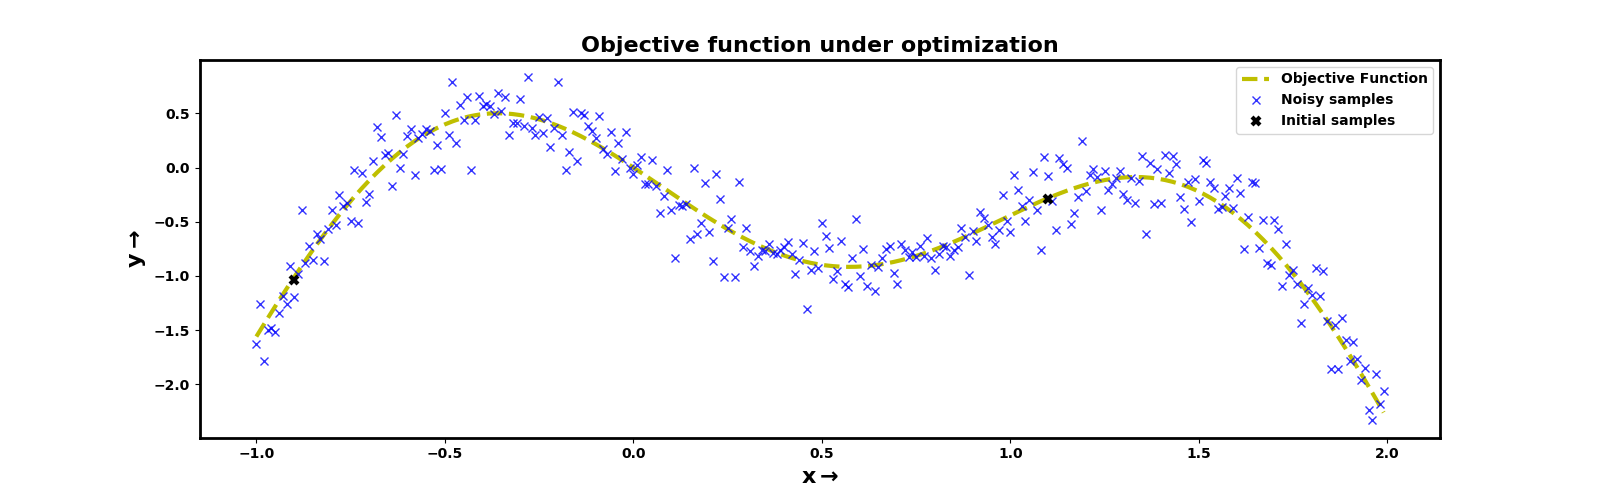
\includegraphics[width=0.8\linewidth,height=0.25\textheight]{images/BO_objective.png}
\captionsetup{justification=justified}
\caption[An example objective function under BO]{An example objective function to illustrate the working of Bayesian optimization.}
\label{fig:BO_objective}
\end{figure}

\begin{figure}[!ht]
		\centering
		\begin{subfigure}{1\textwidth}
  			\centering
  			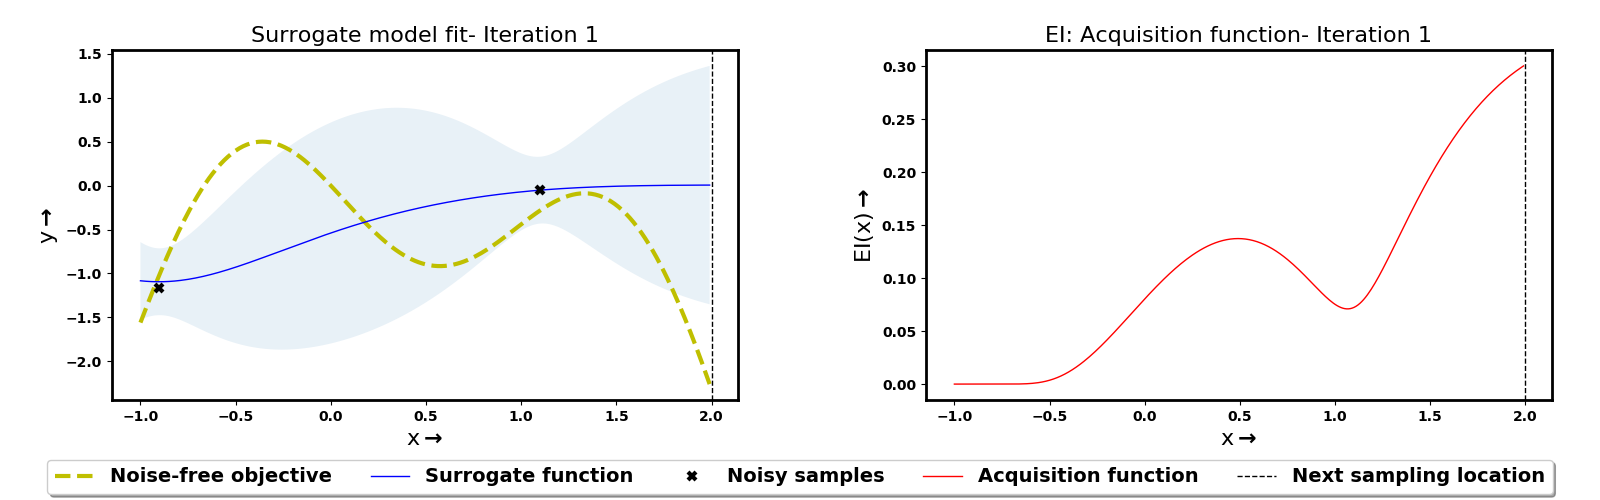
\includegraphics[width=1\linewidth, height=0.2\textheight]{images/BO1.png}
  			\caption{Evaluate the query points (EVALUATE) $\rightarrow$Fit surrogate to initial evaluation (FIT)$\rightarrow$ Maximize EI to find the next query point (MAXIMIZE EI).}
  			\label{fig:BO1}
		\end{subfigure}
		\begin{subfigure}{1\textwidth}
  			\centering
  			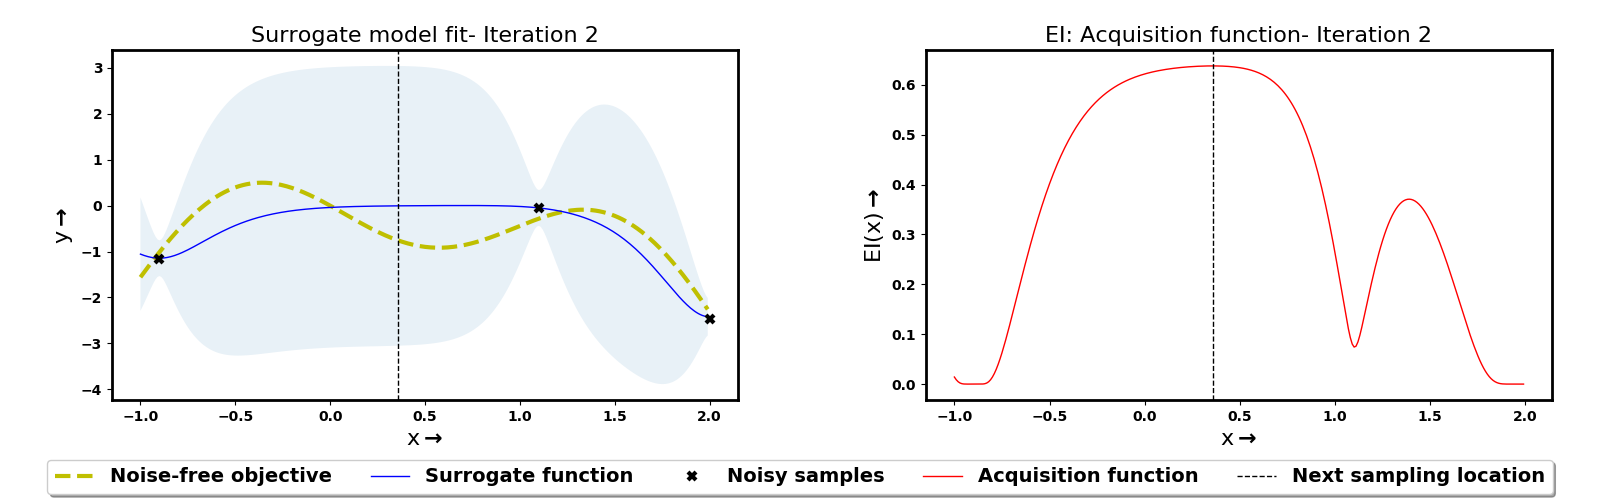
\includegraphics[width=1\linewidth, height=0.2\textheight]{images/BO2.png}
  			\caption{EVALUATE $\rightarrow$ FIT $\rightarrow$ MAXIMIZE EI.}
  			\label{fig:BO2}
		\end{subfigure}
		\begin{subfigure}{1\textwidth}
  			\centering
  			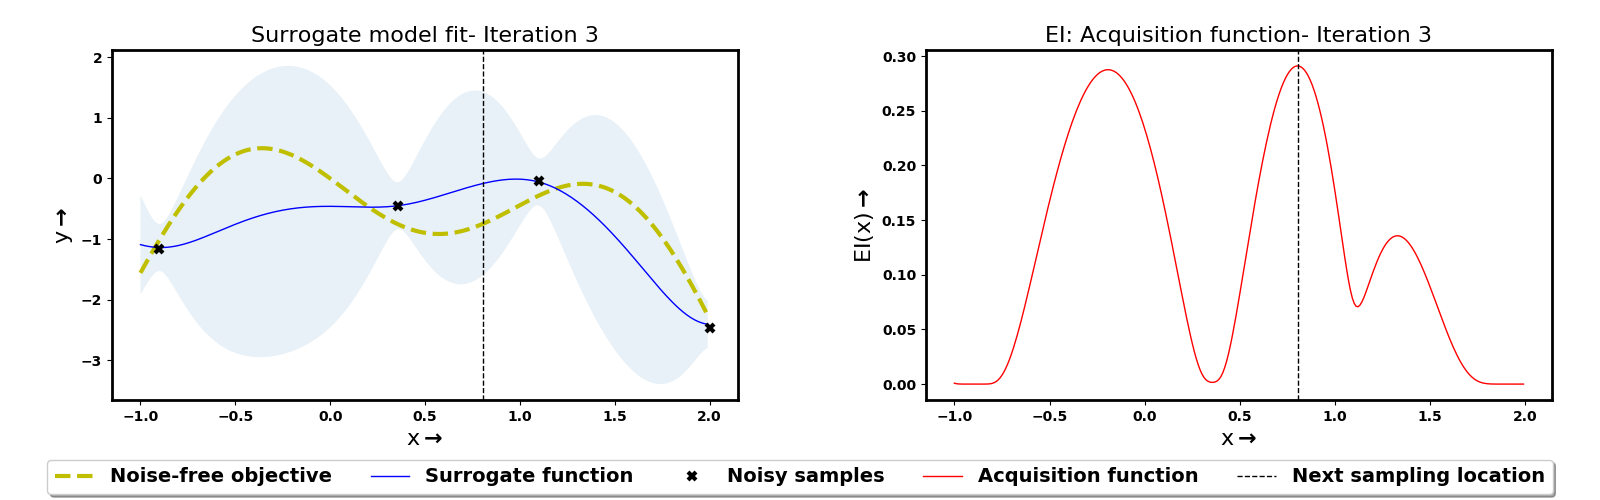
\includegraphics[width=1\linewidth, height=0.2\textheight]{images/BO3.png}
  			\caption{EVALUATE $\rightarrow$ FIT $\rightarrow$ MAXIMIZE EI.}
  			\label{fig:BO3}
		\end{subfigure}
		\begin{subfigure}{1\textwidth}
  			\centering
  			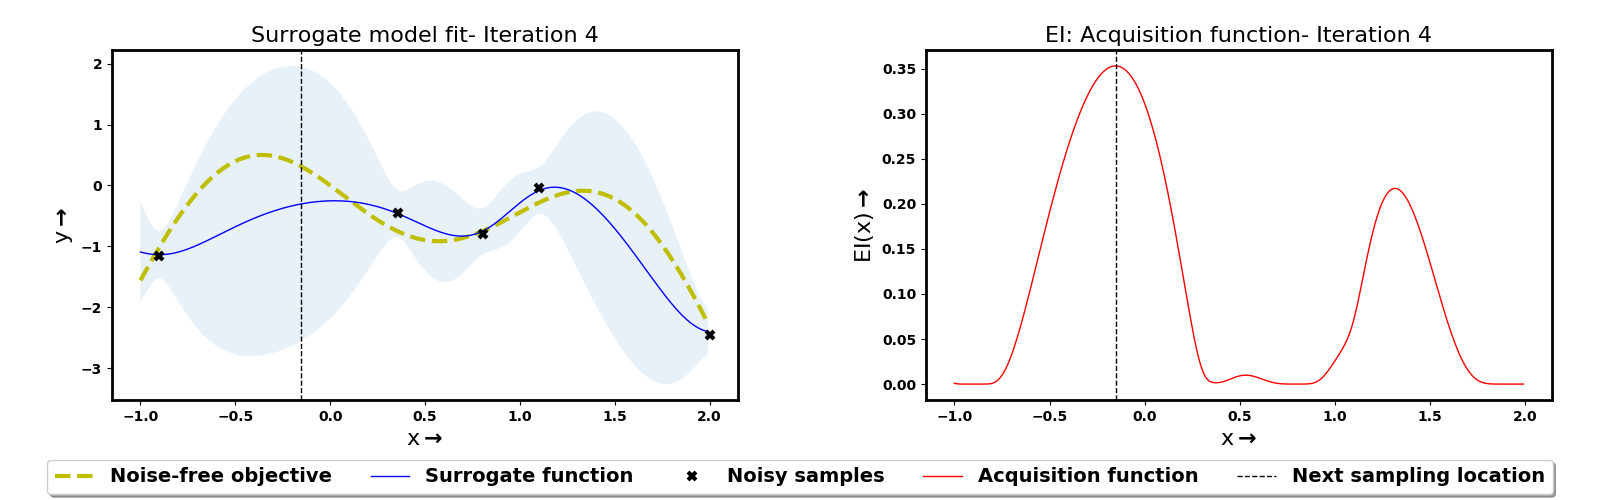
\includegraphics[width=1\linewidth, height=0.2\textheight]{images/BO4.png}
  			\caption{EVALUATE $\rightarrow$ FIT $\rightarrow$ MAXIMIZE EI.}
  			\label{fig:BO4}
		\end{subfigure}
\captionsetup{justification=justified}
\caption[Illustration of BO- Iterations 1 to 4.]{Illustration of BO- Iterations 1 to 4.}
\label{fig:BO_steps}
\end{figure}


\begin{figure}[!ht]
		\centering
		\begin{subfigure}{1\textwidth}
  			\centering
  			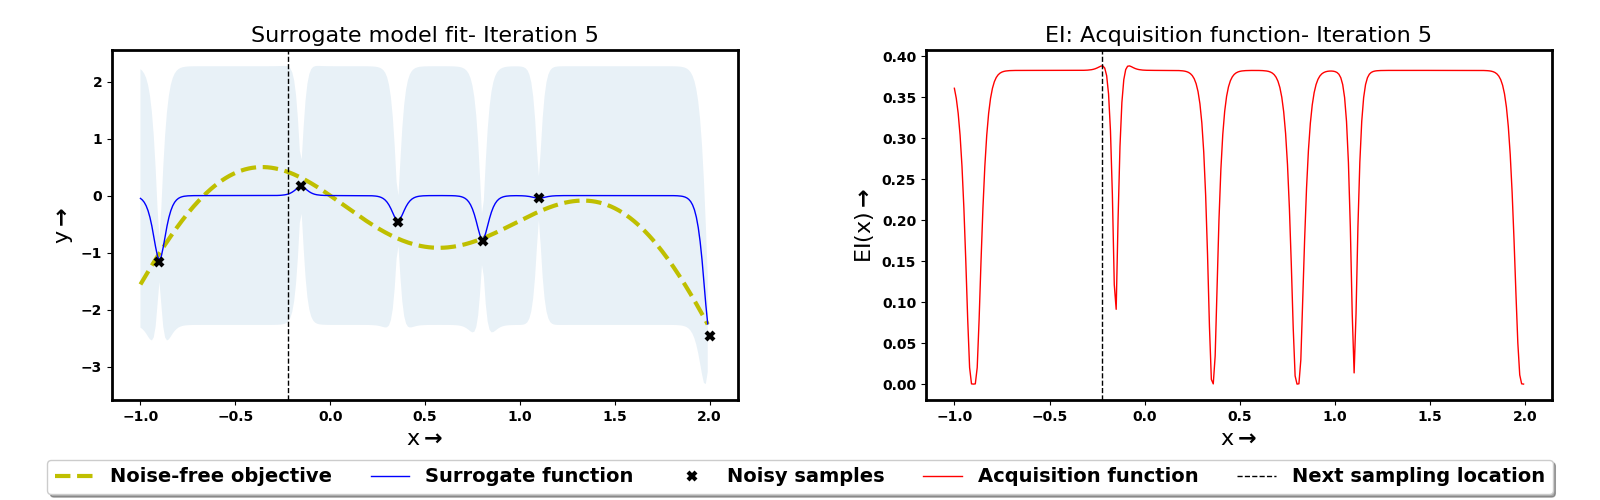
\includegraphics[width=1\linewidth, height=0.2\textheight]{images/BO5.png}
  			\caption{EVALUATE $\rightarrow$ FIT $\rightarrow$ MAXIMIZE EI.}
  			\label{fig:BO5}
		\end{subfigure}
		\begin{subfigure}{1\textwidth}
  			\centering
  			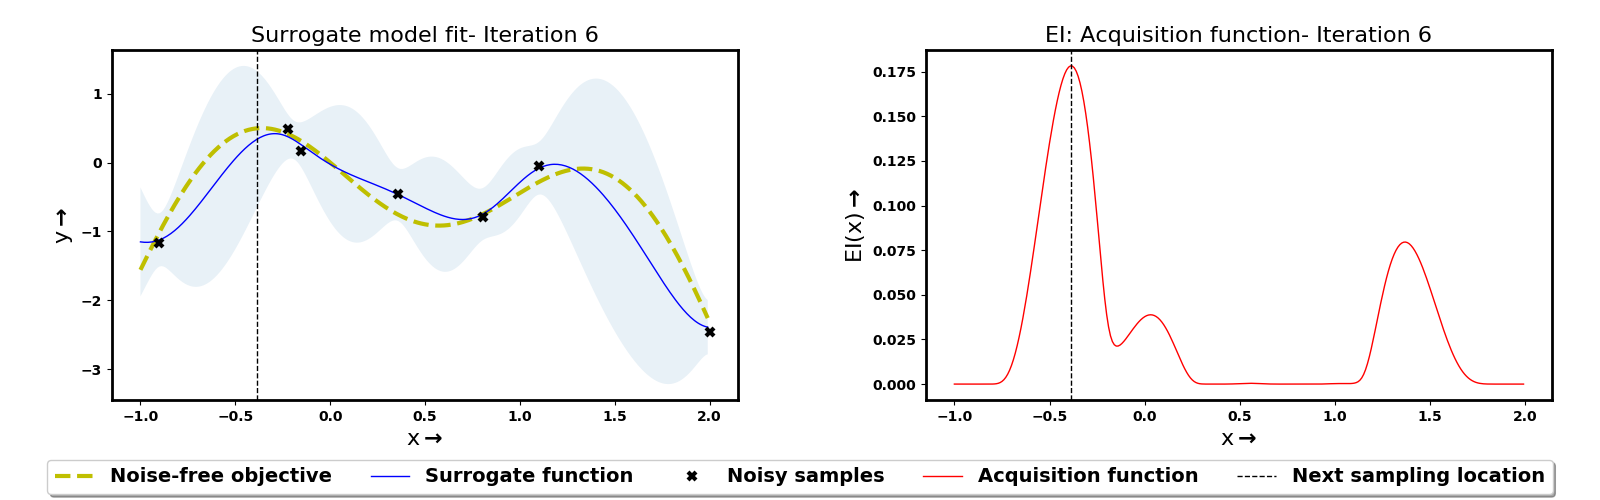
\includegraphics[width=1\linewidth, height=0.2\textheight]{images/BO6.png}
  			\caption{EVALUATE $\rightarrow$ FIT $\rightarrow$ MAXIMIZE EI.}
  			\label{fig:BO6}
		\end{subfigure}
		\begin{subfigure}{1\textwidth}
  			\centering
  			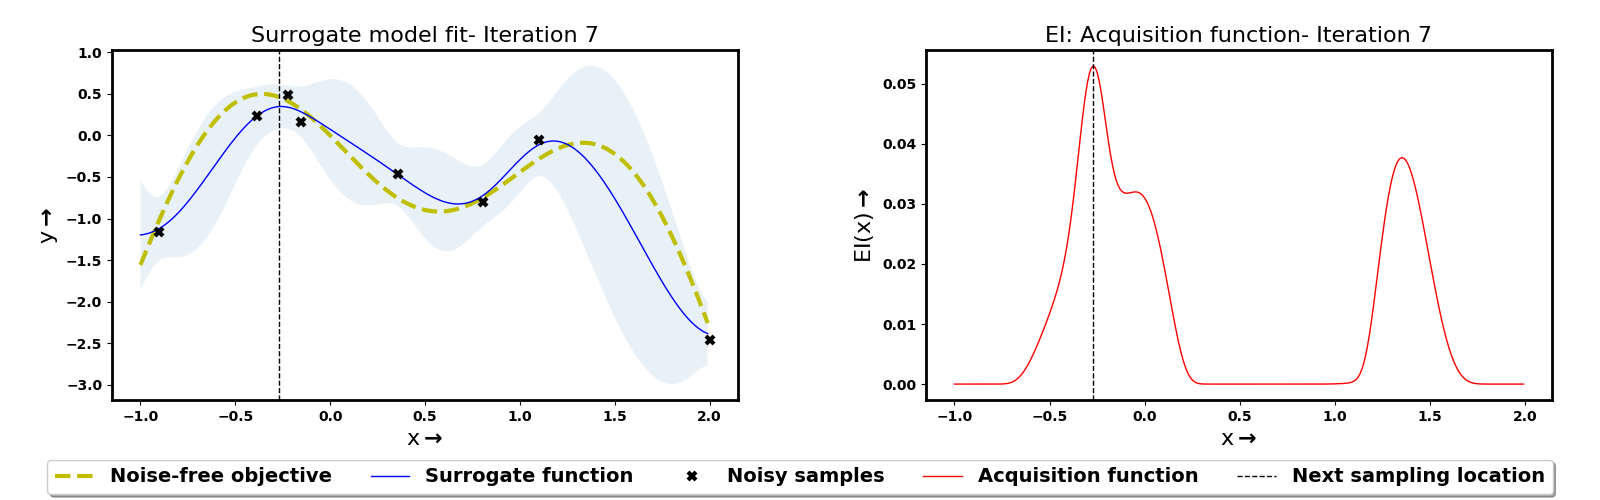
\includegraphics[width=1\linewidth, height=0.2\textheight]{images/BO7.png}
  			\caption{EVALUATE $\rightarrow$ FIT $\rightarrow$ MAXIMIZE EI.}
  			\label{fig:BO7}
		\end{subfigure}
		\begin{subfigure}{1\textwidth}
  			\centering
  			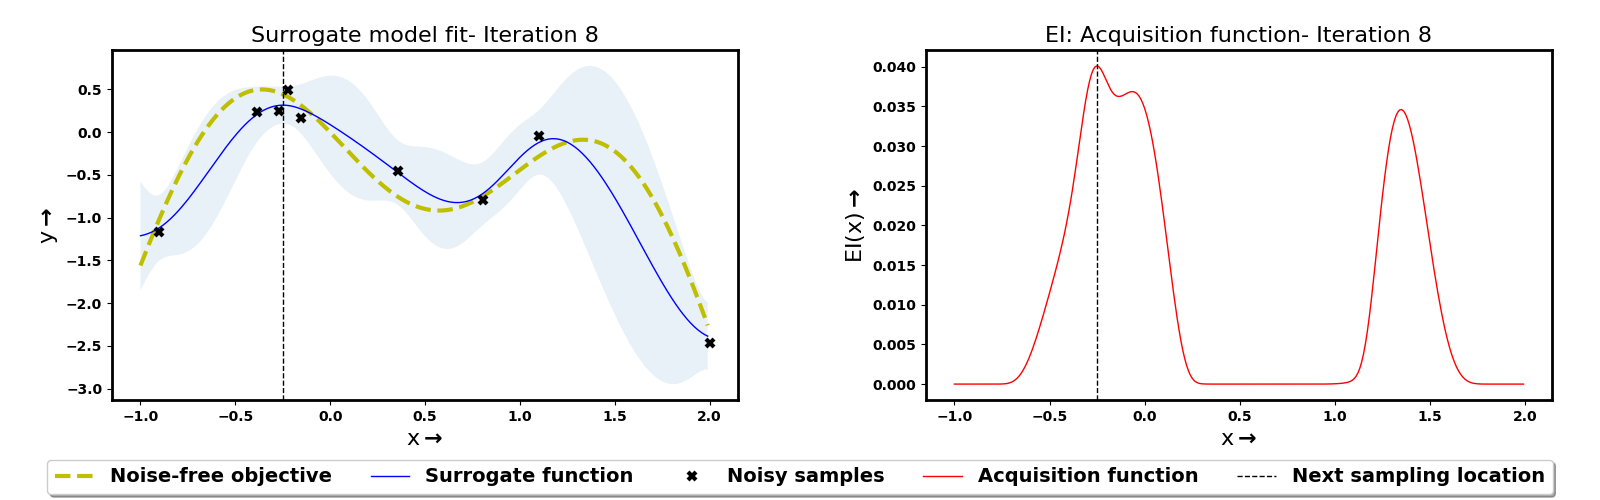
\includegraphics[width=1\linewidth, height=0.2\textheight]{images/BO8.png}
  			\caption{EVALUATE $\rightarrow$ FIT $\rightarrow$ MAXIMIZE EI. BO terminates returning the best sample point for 8 iterations.}
  			\label{fig:BO8}
			\end{subfigure}
\captionsetup{justification=justified}
\caption[Illustration of BO- Iterations 5 to 8.]{Illustration of BO- Iterations 5 to 8.}
\label{fig:BO_steps2}
\end{figure}

\chapter{Flowchart of SMAC}
\label{chapter:smac_flowchart}

This section explains the flowchart of SMAC. In this research work, SMAC is used to optimize the training and evaluation simulation instances by per-instance black box optimization.  The blue marks indicate the file names performing the task in the smart coupling tool package \ref{appendix:gitlab_package} provided for user convenience. The working of the SMAC is explained in detail at \ref{section:smac_smartcoupling_algorithm}. In \ref{section:smac_smartcoupling_algorithm}, the optimization is explained for all the training instance. In contrast, this section covers single instance optimization by running the smart coupling tool with single MpCCI input file. 

\begin{figure}[!ht]
\centering
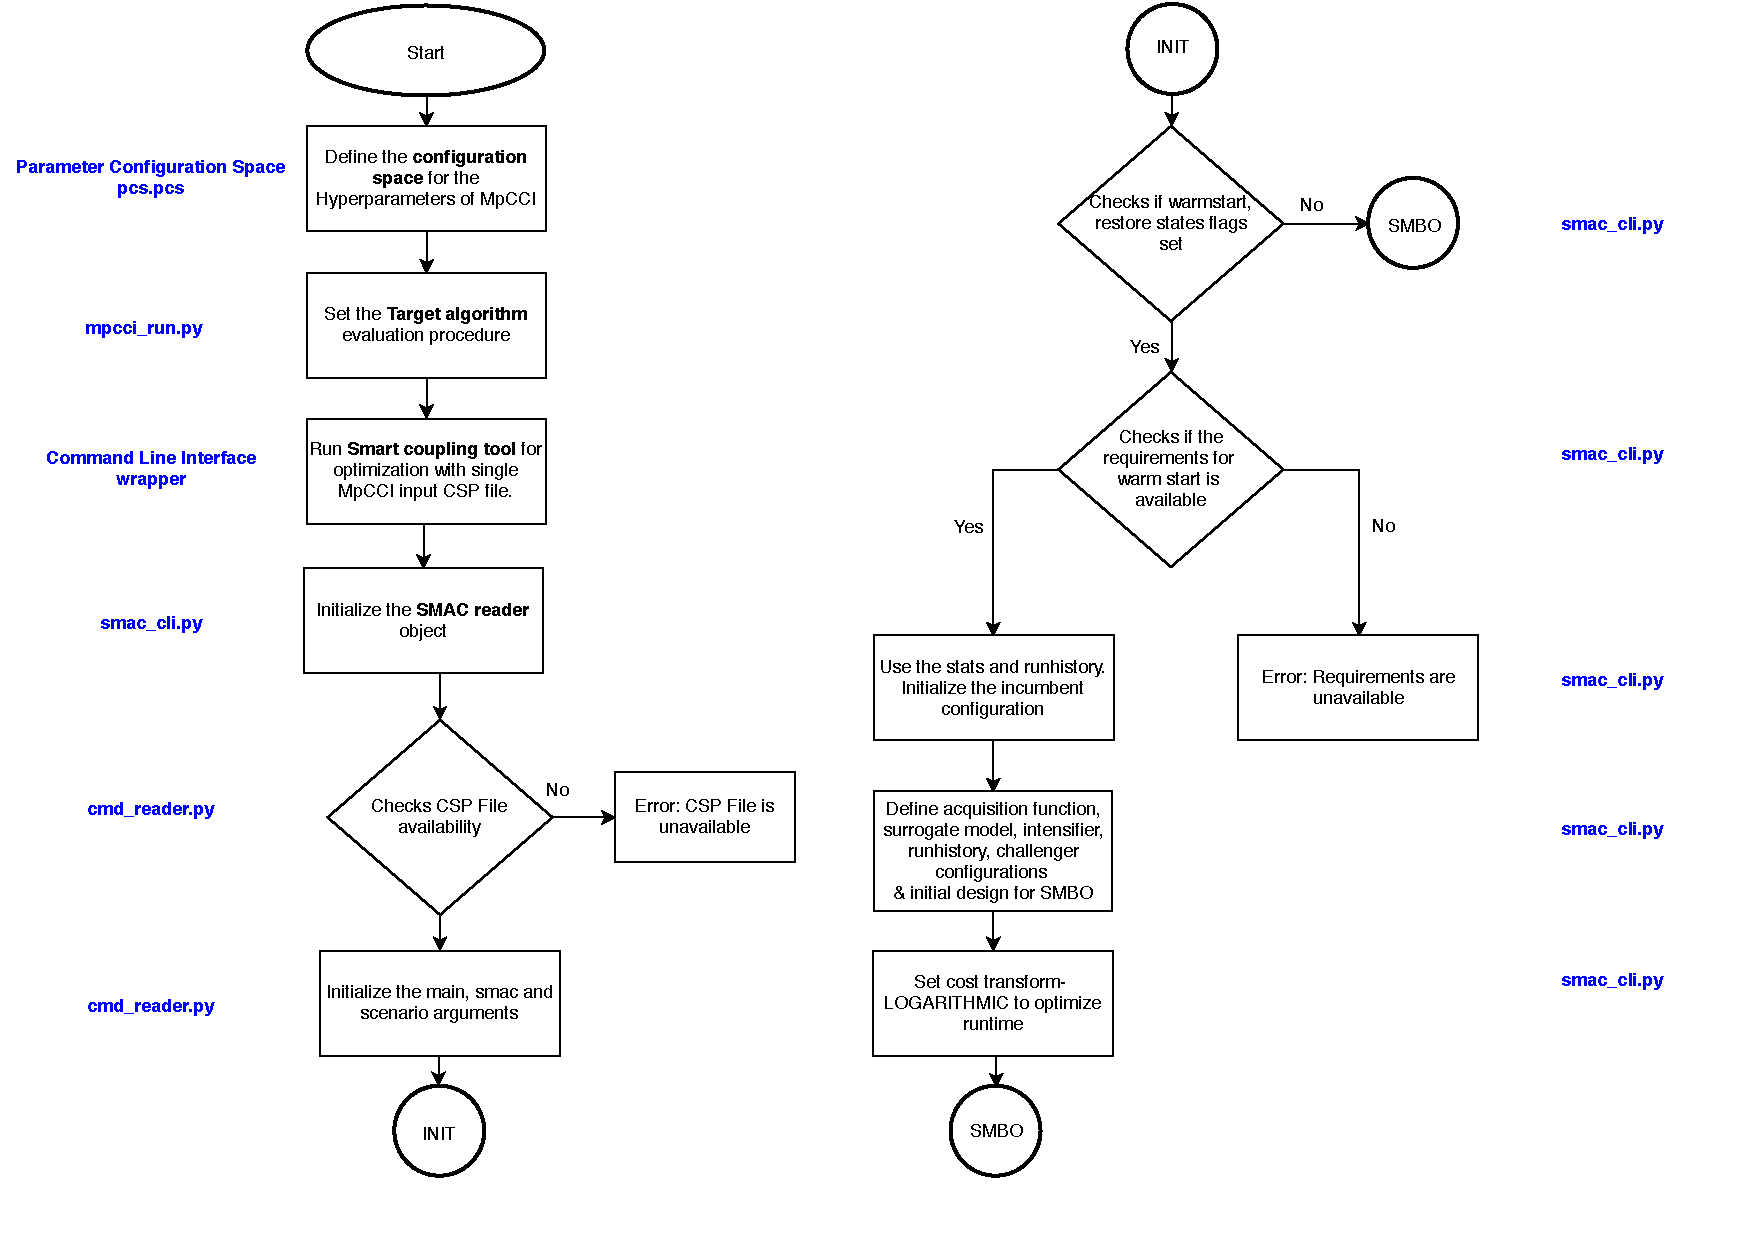
\includegraphics[width=\textwidth,height=0.6\textheight]{images/Flowchart_SMAC-1.pdf}
\captionsetup{justification=justified}
\caption[Flowchart of SMAC- Part 1]{Flowchart of SMAC performing single instance optimization- 1.}
\label{fig:flowchart-smac1}
\end{figure}

\begin{figure}[!ht]
\centering
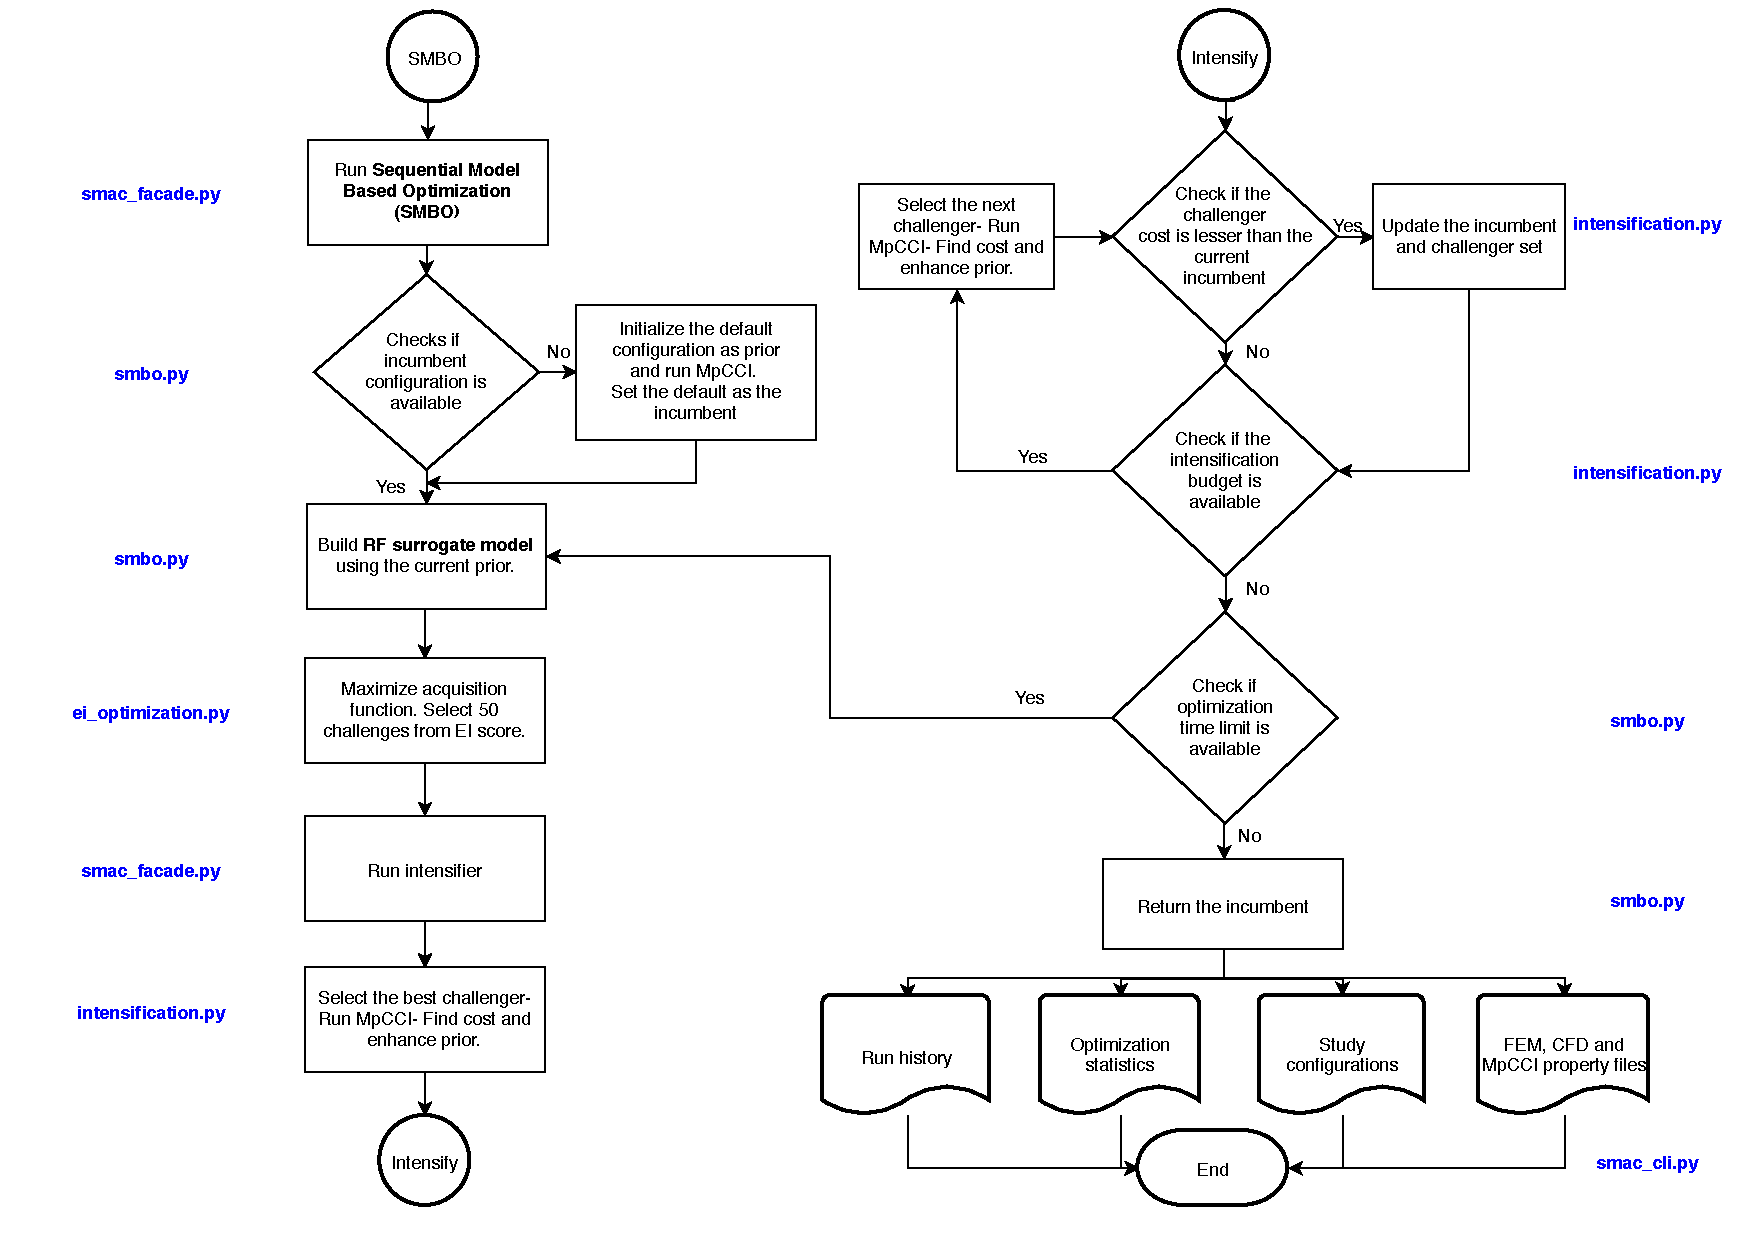
\includegraphics[width=\textwidth,height=0.6\textheight]{images/Flowchart_SMAC-2.pdf}
\captionsetup{justification=justified}
\caption[Flowchart of SMAC- Part 2]{Flowchart of SMAC performing single instance optimization- 2.}
\label{fig:flowchart-smac2}
\end{figure}

\chapter{Software tools contributed}
\label{appendix:gitlab_package}

The python-based packages of the smart coupling and feature reader tools are available in a \href{https://gitlab.scai.fraunhofer.de/deepan.chakravarthi.padmanabhan/smart_coupling/tree/master}{GitLab repository}\footnote{https://gitlab.scai.fraunhofer.de/deepan.chakravarthi.padmanabhan/smart\_coupling/tree/master}. The package holds a private ownership. Kindly contact Mr. Klaus Wolf\footnote{Email ID: klaus.wolf@scai.fraunhofer.de} and Mr. Hamid Arjmandi\footnote{Email ID: hamid.reza.arjmandi.marvast@scai.fraunhofer.de} for collaboration.

\section{Smart coupling tool}
\label{appendix:smart_coupling_tool}
The smart coupling tool provides a suitable configuration for a co-simulation given the MpCCI simulation input files. The MpCCI input files and the process of setting up MpCCI is available at \cite{MpCCI_documentation}. The package operates in three different phases- Optimization, Training and Prediction. This package includes an implementation of the original SMAC from \cite{smac-github} developed by the Marius Lindauer, Katharina Eggensperger, Matthias Feurer, Stefan Falkner, André Biedenkapp and Frank Hutter. However, the SMAC has been modified using the algorithm \ref{algo:smac}. The steps to utilize the package are enumerated below. 

\begin{enumerate}
\item Clone the repository  \href{https://gitlab.scai.fraunhofer.de/deepan.chakravarthi.padmanabhan/smart_coupling/tree/master}{Smart coupling tool and feature reader}. 
\item The initial requirement is swig (4.0 $>=$ 3.0, recommended 3.0.12). Next, install all the requirements to use the package using the below commands. 

\textbf{\$ $\text{cat requirements.txt $|$ xargs -n 1 -L 1 pip install}$}
\newline
\noindent \textbf{\$ $\text{ pip install .} $}

\item Optimization phase: The optimization phase optimizes a given simulation problem and the output contains the run history of the optimization, the best configuration for the particular simulation instance and the features of the simulation instance.

\textbf{\$ $ \text{mpcci\_smac --csp $<$csp-file.csp$>$ --pcs $<$pcs-file.pcs$>$ } $}

\text{$<$csp-file.csp$>$} is the MpCCI project input file. \text{$<$pcs-file.pcs$>$} is the parameter configuration space format file containing the range and default values of the parameters. The MpCCI project file holds all the information regarding the co-simulation task- the solid and fluid model files directory and coupling parameters required from the user.

\item Training phase: The training phase trains the machine learning models for all the simulation instances optimized. The dataset is created online given the run history and features of the simulation instances. The run history and features of the simulation are present in the output directory of the optimization phase. Therefore, this phase requires only the output of the optimization phase of each instance.

\textbf{\$ $\text{mpcci\_smac --mode TRAIN --trainstudy $<$trainstudy-file.txt$>$}$}

\text{$<$trainstudy-file.txt$>$} contains the mpcci\_smac optimization phase output directory of all the training instances.

\item Prediction phase: The prediction phase utilize the models trained in the training phase. In addition, it uses the user provided MpCCI input csp files and the pcs files.

\textbf{\$ $\text{mpcci\_smac --mode PREDICT --csp $<$csp-file.csp$>$ --pcs\textbackslash}$}
\newline
\textbf{ $\text{ $<$pcs-file.pcs$>$ --models $<$path-of-trained-models$>$}$}

The output of the prediction phase is the MpCCI input files with the configurations predicted by the smart coupling tool for the simulation instance provided by the user.

% \begin{figure}[!htp]
% \centering
% 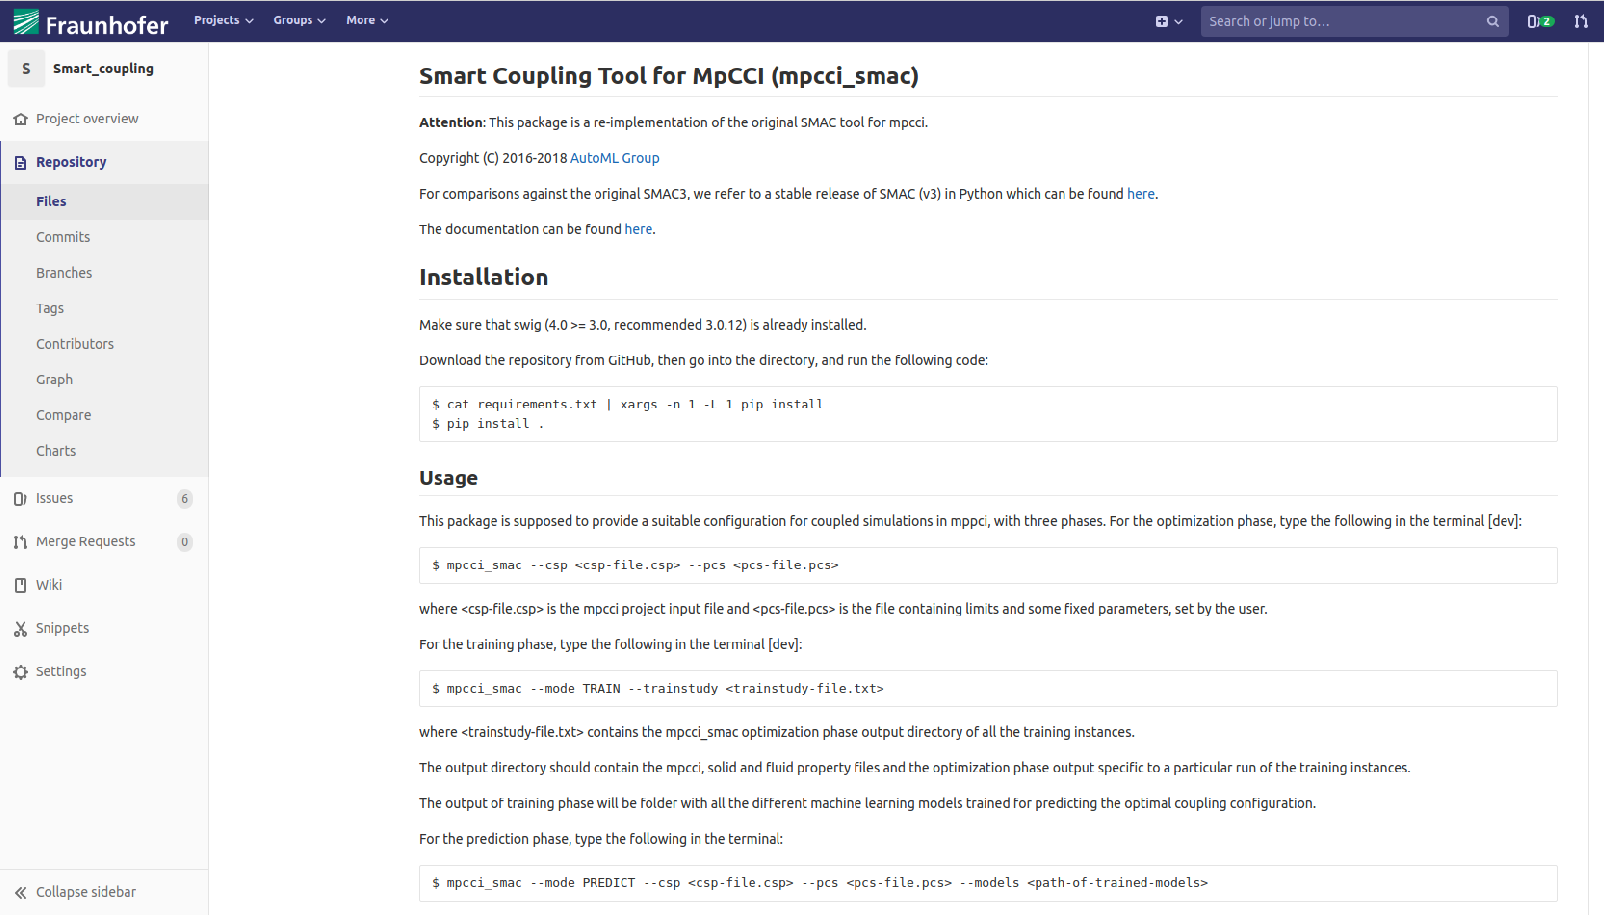
\includegraphics[width=\textwidth,height=0.5\textheight]{images/tool.png}
% \captionsetup{justification=justified}
% \caption[Smart coupling tool- GitLab screenshot]{Smart coupling tool- GitLab screenshot.}
% \label{fig:mpcci_smac_github}
% \end{figure}
\end{enumerate}

\section{Feature reader}
\label{appendix:feature_reader}
The feature reader package provides the features of the simulation instance. It extracts approximately 100 features from the solid and fluid simulation models, MpCCI inputs and the result log of MpCCI. For this research purpose only 6 features are used depending on the literature study \cite{FSI_properties} \cite{FSI_properties2}. The package installation is similar to smart coupling tool. The following command executes the feature reader.

\noindent \textbf{\$ $\text{mpcci\_feature\_reader $<$csp-file.csp$>$ $<$mpcci-job-file.log$> $\textbackslash}$}
\newline
\textbf{$\text{ $<$mpcci-server-file.log$>$}$}

\chapter{COSEAL 2019 poster}
\label{chapter:coseal_poster}

This research work was selected for poster presentation at the \href{https://www.coseal.net/coseal-workshop-2019/}{COnfiguration and SElection of ALgorithms workshop 2019} held at Potsdam, Berlin on 26th and 27th August 2019. It was organized by experts in the field of Automated Algorithm Configuration, Prof. Dr. Holger H. Hoos and M. Sc. Marius Lindauer. The poster is included in the following page. 


% \chapter{Miscellaneous plots}

% \begin{figure}[!ht]
% \centering
% 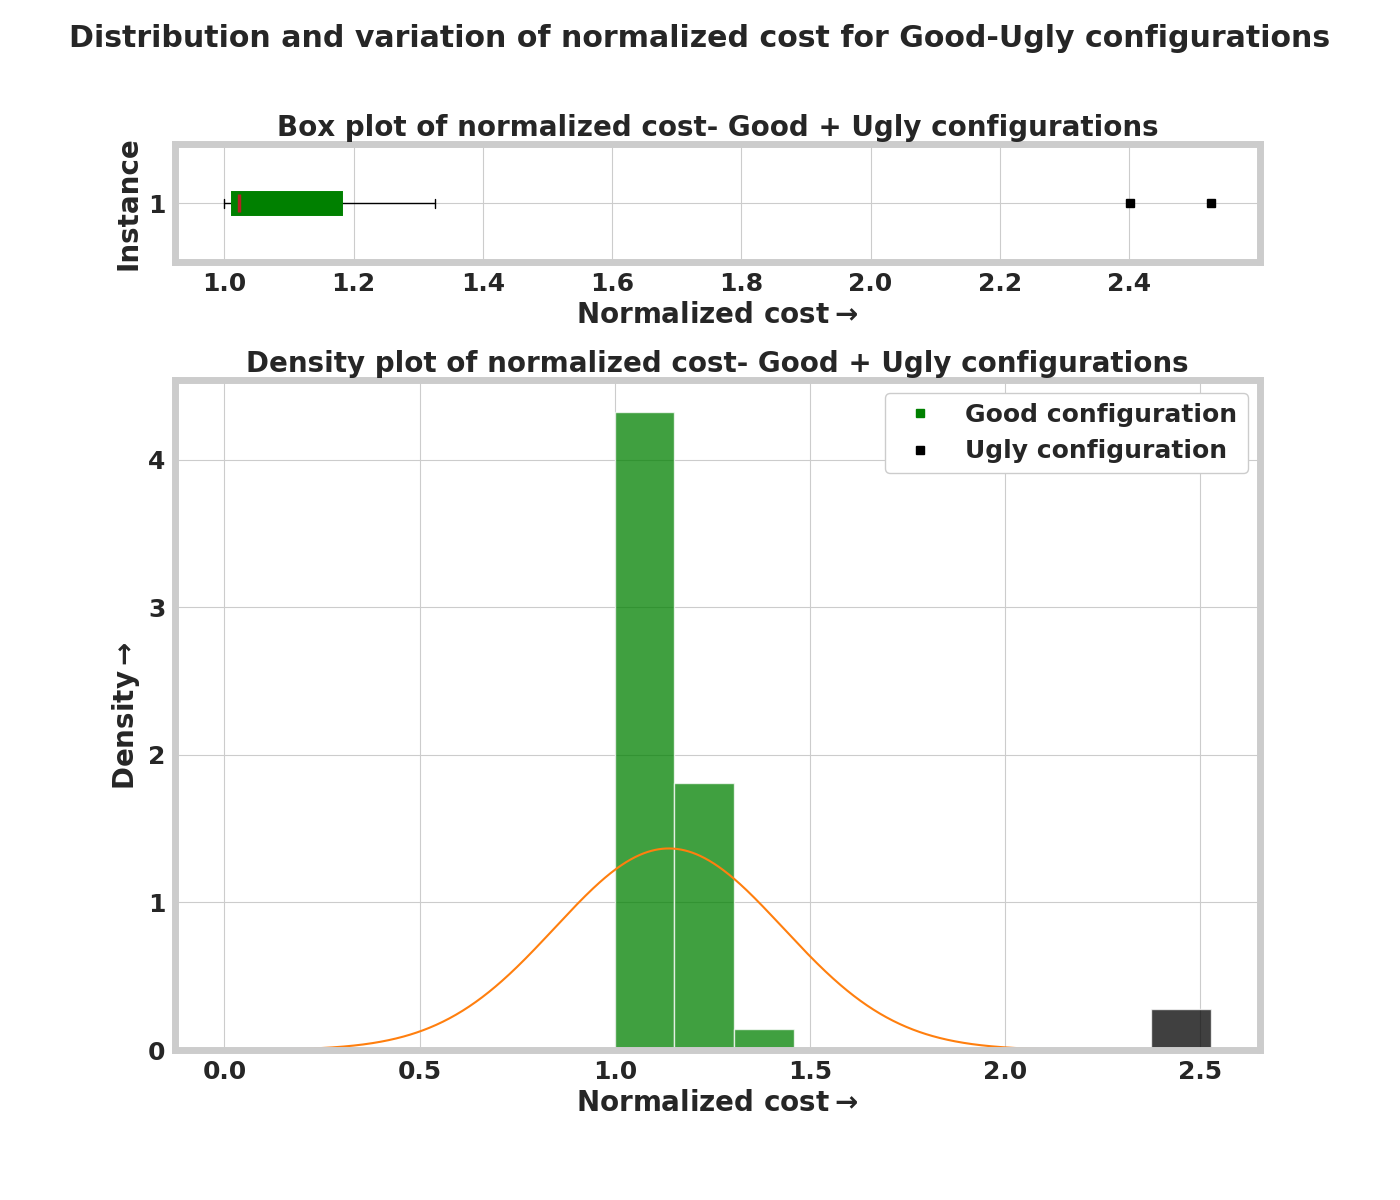
\includegraphics[width=1\linewidth,height=0.4\textheight]{images/Good_ugly_dist.png}
% \captionsetup{justification=centering}
% \caption{Cost and configuration response model training and prediction phase. }
% \label{fig:training_prediction}
% \end{figure}